\documentclass{classrep}
\usepackage[utf8]{inputenc}
\frenchspacing

\usepackage{graphicx}
\usepackage[usenames,dvipsnames]{color}
\usepackage[hidelinks]{hyperref}
\usepackage{lmodern}
\usepackage{graphicx}
\usepackage{placeins}
\usepackage{url}
\usepackage{amsmath, amssymb, mathtools}
\usepackage{listings}
\usepackage{fancyhdr, lastpage}
\usepackage{listings}

%New colors defined below
\definecolor{codegreen}{rgb}{0,0.6,0}
\definecolor{codegray}{rgb}{0.5,0.5,0.5}
\definecolor{codepurple}{rgb}{0.58,0,0.82}
\definecolor{backcolour}{rgb}{0.95,0.95,0.92}

%Code listing style named "mystyle"
\lstdefinestyle{mystyle}{
    commentstyle=\color{codegreen},
    keywordstyle=\color{magenta},
    numberstyle=\tiny\color{codegray},
    stringstyle=\color{codepurple},
    basicstyle=\tiny,
    breakatwhitespace=false,
    breaklines=true,
    captionpos=b,
    keepspaces=true,
    numbers=left,
    numbersep=5pt,
    showspaces=false,
    showstringspaces=false,
    showtabs=false,
    tabsize=2
}

%"mystyle" code listing set
\lstset{style=mystyle}

\pagestyle{fancyplain}
\fancyhf{}
\renewcommand{\headrulewidth}{0pt}
\cfoot{\thepage\ / \pageref*{LastPage}}

%--------------------------------------------------------------------------------------%
\studycycle{Informatyka, studia dzienne, inż I st.}
\coursesemester{VI}

\coursename{Sztuczna inteligencja i systemy ekspertowe}
\courseyear{2019/2020}

\courseteacher{dr inż. Krzysztof Lichy}
\coursegroup{wtorek, 12:15}

\author{%
    \studentinfo{Jan Karwowski}{216793}\\
    \studentinfo{Kamil Kowalewski}{216806}%
}

\title{Zadanie 2: Sieć neuronowa do korygowania pomiaru systemu lokalizacji}

\begin{document}
    \maketitle
    \thispagestyle{fancyplain}

    \section{Opis architektury sieci neuronowej} {

        W realizacji zadania wykorzystana została architektura sieci neuronowej znana jako
        perceptron wielowarstwowy MLP. W warstwach przetwarzających (wszystkich poza pierwszą),
        funkcja aktywacji zawsze jest sigmoidalna. Wykonanych zostało bardzo wiele (dziesiątki)
        eksperymentów, mających na celu znalezienie właściwej architektury sieci, pozwalającej jak
        najbardziej minimalizować błąd. Wyniki dla tych układów neuronów, które w ogóle udało się
        czegoś nauczyć, nie różniły się bardzo między sobą. Zbadane zostały układy wykorzystujące od
        kilku do kilkunastu ostatnich pomiarów, gdzie neuronów w jednej lub dwóch warstwach ukrytych
        również było kilka, lub maksymalnie kilkanaście.

        Zauważono, że generalnie należy wykorzystywać więcej niż 3 ostatnie pomiary, ale z kolei
        przy zbyt dużej ich liczbie (prawie 10) trudno jest już wyuczyć sieć. Dodatkowo okazało się,
        że lepsze wyniki uzyskane zostały dla dwóch warstw ukrytych niż jednej, nawet jeżeli jedna
        ma kilkanaście neuronów, a dwie mają po kilka. Generalnie, jak już wspomniano powyżej,
        wyniki otrzymywane dla różnych architektur nie różniły się bardzo, natomiast niektóre
        rzeczywiście można było uznać za poprawiające wyniki pomiarów pozycji robota, a inne
        zdecydowanie pomiarów nie poprawiały, wręcz przeciwnie - zniekształcały. Ostatecznie wybrana
        została jedna architektura, którą uznano za zdecydowanie (choć niewiele) poprawiającą wyniki
        pomiarów pozycji. Oczywiście nie jest to najlepsze możliwe rozwiązanie, gdyż wyniki
        poprawiają się dla coraz to bardziej złożonych sieci (więcej warstw i/lub neuronów),
        bardziej złożone sieci jest jednak trudniej uczyć a ponadto trwa to znacznie dłużej. Wybrana
        architektura jest więc jedną z lepszych ale tylko spośród tych, które udało się przebadać.
        Należy wspomnieć jeszcze o tym, że wynik procesu uczenia danej architektury i w konsekwencji
        jakość poprawy błędów pomiaru są w jakimś stopniu zależne od początkowych wag neuronów,
        które są dobierane w sposób losowy.  Oznacza to, że w zależności od tego początkowego
        losowania, dana architektura może sprawdzić się troche lepiej lub trochę gorzej, a w
        skrajnych przypadkach znacznie gorzej.  Poniżej dokładny opis wybranej architektury
        perceptronu wielowarstwego, wraz z wartościami wag dla każdego neuronu w każdej warstwie.

        \begin{itemize}
            \item liczba próbek z poprzednich chwil czasowych - 4
            \item liczba warstw sieci - 4
            \item warstwa 1. - 8 neuronów (warstwa nieprzetwarzająca)
            \item warstwa 2. - 6 neuronów (funkcja aktywacji sigmoidalna)
            \item warstwa 3. - 6 neuronów (funkcja aktywacji sigmoidalna)
            \item warstwa 4. - 2 neurony (funkcja aktywacji sigmoidalna)
        \end{itemize}

        \begin{table}[!htbp]
            \centering
            \begin{tabular}{|c|c|c|c|c|c|l|}
            \hline
            & Neuron 1      & Neuron 2      & Neuron 3       \\ \hline
     Waga 1 & 2.527598267340922              &  -0.17441081463297675             &  1.6363204100359892              \\ \hline
     Waga 2 & -0.9232272541113129              & -1.6980059145632285              & -2.6032578398626907               \\ \hline
     Waga 3 & -0.3984130671505576              & -1.7499693315083193              & -2.8195104269688653               \\ \hline
     Waga 4 & -0.569507339062675              &  -1.5062334750638877             &  -2.6600809245045256              \\ \hline
     Waga 5 & -0.4607775220073911              & -1.9820533887145988              &  -2.6777819113221684              \\ \hline
     Waga 6 & -2.541843352618611              & 0.17569149828227681              & 1.1873074117628548               \\ \hline
     Waga 7 & -1.9395361323975755              & 0.1511906068644519              &  1.2127143947430732              \\ \hline
     Waga 8 & -1.8524104808108466              & 0.14654460888562296              &  1.111583615125505              \\ \hline
     Waga 9 & -1.9771371527335988              & 0.0546662863936919              &  1.1599139025156642              \\ \hline

            \end{tabular}
            \caption{Warstwa numer 2}
        \end{table}
        \FloatBarrier

        \begin{table}[!htbp]
            \centering
            \begin{tabular}{|c|c|c|c|c|c|l|}
            \hline
                   & Neuron 4      & Neuron 5      & Neuron 6        \\ \hline
            Waga 1 &  2.363638180205667             & 3.8376271260920505              & -0.9484892877372848                \\ \hline
            Waga 2 & -2.0185244724902165              & -0.9130778067081949              & 0.8246073479256618                \\ \hline
            Waga 3 & -1.6725622011445482              & -1.1990399152120987              & 0.3471172778041218                \\ \hline
            Waga 4 & -1.6560041428219832              & -1.0356331937638623              & 0.31316040546212776                \\ \hline
            Waga 5 & -1.694781898940903              &  -1.0447150859638734             & 0.061197474417249056                \\ \hline
            Waga 6 & 1.7020218973634886              & -1.437916680812331              & 0.1596894645232247                \\ \hline
            Waga 7 & 1.6992915302904315              & -1.087790023686115              & 0.5111741427023013                \\ \hline
            Waga 8 & 1.8281281031432608              & -1.05147303362551              &  0.5531791532256888               \\ \hline
            Waga 9 & 1.918453443921396              & -1.1752781948210815              & 0.4576405425211791                \\ \hline

            \end{tabular}
            \caption{Warstwa numer 2 (cd.)}
            \end{table}
        \FloatBarrier


        \begin{table}[!htbp]
            \centering
            \begin{tabular}{|c|c|c|c|c|c|l|}
            \hline
                    & Neuron 1      & Neuron 2      & Neuron 3        \\ \hline
            Waga 1 & -0.54104637866259              &  -1.7068531839763332             & 0.4660004428963209                \\ \hline
            Waga 2 & 1.3917794904558363              & -1.815146068655716              & 0.302406328502846                \\ \hline
            Waga 3 & -1.2412118399681937              & 2.2897514884650905              & -3.1060163015774505                \\ \hline
            Waga 4 & -3.2329287168978396              & 1.497185122036276              & -3.1859032863902157                \\ \hline
            Waga 5 & -0.5677394310707327              & 0.05551820938295718              & -4.683123646942736                \\ \hline
            Waga 6 & 0.3346563062731672              &  0.1519129480587903             &  -3.6759099132364867               \\ \hline
            Waga 7 & -0.3533554672232843              & -1.7825267801136424              & 0.49067055329904785                \\ \hline

            \end{tabular}
            \caption{Warstwa numer 3}
            \end{table}
        \FloatBarrier


        \begin{table}[!htbp]
            \centering
            \begin{tabular}{|c|c|c|c|c|c|l|}
            \hline
                   & Neuron 4      & Neuron 5      & Neuron 6        \\ \hline
            Waga 1 & -0.6808869300654189              & 0.3565561020683462              & -2.304122968112266                \\ \hline
            Waga 2 & -0.4890807542347913              & -2.751084125263123              & 1.067886336171889                \\ \hline
            Waga 3 & 0.9777191106201556              & 0.22732150887581046              & 2.00842165374729                \\ \hline
            Waga 4 & 1.017403810312005              & 3.404000568004232              & 2.851192563621574                \\ \hline
            Waga 5 & -0.5950758846368603              & -1.7237122060063044              & 0.23063569685649307                \\ \hline
            Waga 6 & -0.632335615114227              & -3.0468660975678428              & 2.457868195279637                \\ \hline
            Waga 7 & -1.0787080615548403              & 0.614108893444899              & -1.454923012685576                \\ \hline

            \end{tabular}
            \caption{Warstwa numer 3 (cd.)}
            \end{table}
        \FloatBarrier


        \begin{table}[!htbp]
            \centering
            \begin{tabular}{|c|c|c|c|c|c|l|}
            \hline
                    & Neuron 1                          & Neuron 2                               \\ \hline
            Waga 1 & 0.6459224130549093              &  0.013059929882749937              \\ \hline
            Waga 2 & 0.6584145536993913              &  -2.3885915189811047              \\ \hline
            Waga 3 & -2.7936694235126787              &  0.36084494007403795              \\ \hline
            Waga 4 & 4.208977136115515                  &   -2.9755424899909655             \\ \hline
            Waga 5 & -0.7996327680600376              & 0.2494870707756161               \\ \hline
            Waga 6 & 0.39678903876665367              &  2.698493711926569              \\ \hline
            Waga 7 & -1.9630736456645195              &  -1.4757795816059005              \\ \hline

            \end{tabular}
            \caption{Warstwa numer 4}
            \end{table}
        \FloatBarrier

    }
%--------------------------------------------------------------------------------------%
    \section{Opis algorytmu uczenia sieci neuronowej} {
        Jako algorytm uczenia sieci neuronowej wykorzystany został popularny \emph{back
        propagation}.  Jest to najczęściej wykorzystywana metoda uczenia klasycznego perceptronu
        wielowarstwowego, w którym mamy do czynienia z funkcjami aktywacji sigmoidalnymi. Podstawą
        działania tej metody jest minimalizacja funkcji kosztu, zdefiniowanej jako suma kwadratów
        różnic wyjść faktycznych i oczekiwanych w sieci:
        \begin{equation}
            \textrm{err} = \sum_{i = 1}^{m}(z_i - y_i)^2
        \end{equation}
        gdzie $m$ - numer wyjścia warstwy sieci, $z_i$ - oczekiwana wartość, $y_i$ - otrzymana
        wartość. Do minimalizacji tej funkcji wykorzystuje się metodę gradientową, gdzie liczy się
        pochodne cząstkowe po wagach neuronów i tak powstały gradient, wykorzystuje się, aby zmienić
        wartości wag w 'kierunku' minimaliacji funkcji. Choć jest to metoda szybka i dająca dobre
        wyniki, pozostaje podatna na lokalne minima, w których może utknąć.

        Opisana powyżej minimalizacja funkcji kosztu jest wykonywana dla wszystkich warstw
        przetwarzających perceptronu. Problemem jest więc wyznaczenie wartości błędu w warstwach
        ukrytych, gdyż początkowo jest on znany jedynie w warstwie ostatniej - podczes uczenia
        nadzorowanego wiadome sę jedynie wartości wyjściowe całej sieci a nie poszczególnych warstw.
        Problem ten jest rozwiązany właśnie przez metodę \emph{back propagation}, która to, jak z
        nazwy wynika, polega na propagowaniu błędu od ostatniej warstwy do pierwszej. Znając błąd
        warstwy $N$, można łatwo obliczyć błąd warstwy $N - 1$ zauważając pewne rekurencyjne
        zależności w pochodnych cząstkowych funkcji kosztu warstw następujących jedna po drugiej.
    }
%--------------------------------------------------------------------------------------%
    \section{Porównanie dystrybuant błędu pomiaru} {

        Poniższe rysunki przedstawiają wyniki działania sieci neuronowej w procesie poprawy błędów
        pomiaru pozycji robota. Pierwszy z nich to wygodna do subiektywnej, wizualnej oceny
        reprezentacja pozycji robota w trzech różnych wersjach - rzeczywistej, zmierzonej i
        poprawionej przez sieć. Widzimy tutaj, że algorytm rzeczywiście w pewnych obszarach znacząco
        poprawia pomiary pozycji. Jednak można także zauważyć takie fragmenty, w których wyniki
        sieci ulegają zniekształceniu i mogą być nawet gorsze, niż faktyczne pomiary. Aby
        obiektywnie ocenić czy uzyskane wyniki w ogóle mogą być przydatne lepsze jest porównanie
        dystrybuant przedstawionych na rysunku drugim. Widzimy tutaj, że następuje niewielka, choć
        zdecydowania zauważalna poprawa jakości pomiaru - więcej pomiarów ma mniejsze błędy.

        \begin{figure}[!htbp]
            \centering
            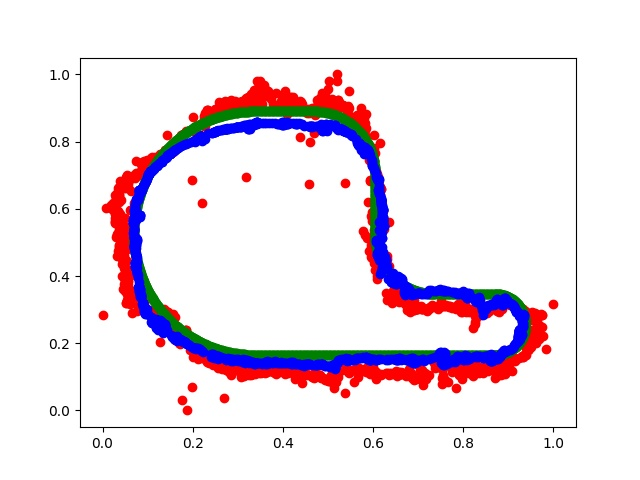
\includegraphics[width=\textwidth]{img/position.jpg}
            \caption{Pozycja robota rzeczywista (zielony), zmierzona (czerwony) i poprawiona przez
            sieć (niebieski)}
        \end{figure}
        \FloatBarrier

        \begin{figure}[!htbp]
            \centering
            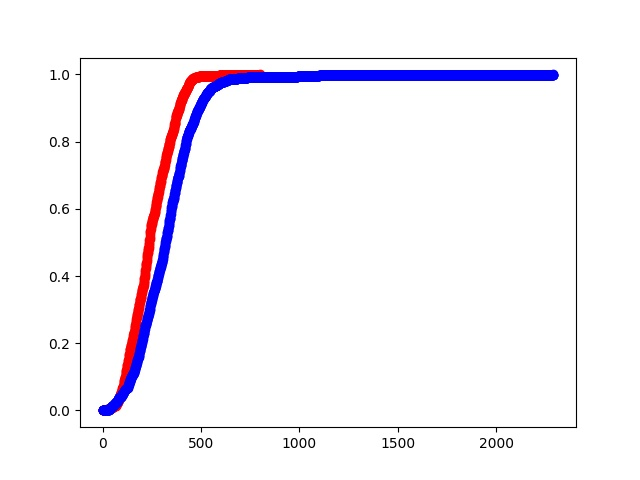
\includegraphics[width=\textwidth]{img/distribution.jpg}
            \caption{Dystrybuant błędy pomiaru przed (niebieski) i po (czerwony) filtracji}
        \end{figure}
        \FloatBarrier
    }
    \newpage
%--------------------------------------------------------------------------------------%

    \section{Kod Źródłowy} \label{kod_zrodlowy} {

        \subsection{Plik główny programu - main.py} {
            \lstinputlisting[language=Python]{source_code/main.py}
        }

        \subsection{Plik Reader.py - wczytywanie danych z plików} {
            \lstinputlisting[language=Python]{source_code/Reader.py}
        }

        \subsection{Plik MLP.py - implementacja sieci neuronowej} {
            \lstinputlisting[language=Python]{source_code/MLP.py}
        }
    }
\end{document}
